\documentclass[12pt]{article}
\usepackage[margin=1in]{geometry} 
\usepackage{amsmath,amsthm,amssymb,amsfonts,algpseudocode,graphicx,mathtools}

\newcommand{\N}{\mathbb{N}}
\newcommand{\Z}{\mathbb{Z}}

\newenvironment{problem}[2][Problem]{\begin{trivlist}
\item[\hskip \labelsep {\bfseries #1}\hskip \labelsep {\bfseries #2.}]}{\end{trivlist}}
%If you want to title your bold things something different just make another thing exactly like this but replace ``problem'' with the name of the thing you want, like theorem or lemma or whatever

\newtheorem{theorem}{Theorem}
\newtheorem{lem}{Lemma}
\DeclarePairedDelimiter{\ceil}{\lceil}{\rceil}

\begin{document}

%\renewcommand{\qedsymbol}{\filledbox}
%Good resources for looking up how to do stuff:
%Binary operators: http://www.access2science.com/latex/Binary.html
%General help: http://en.wikibooks.org/wiki/LaTeX/Mathematics
%Or just google stuff

\title{CMPSCI-683 Homework Assignment \#1: Search}
\author{Patrick Pegus II}
\maketitle

\begin{problem}{1}
	Iterative lengthening search is an iterative analogue of uniform-cost search.
	The basic idea is to use increasing limits on path cost.
	If a node is generated whose path cost exceeds the current limit, it is immediately discarded.
	For each new iteration, the limit is set to the lowest path cost of any node discarded in the previous iteration.
	\begin{enumerate}
		\item Show that this algorithm is optimal for general path costs.

			Let modified uniform-cost path search (MUCS) be uniform-cost search (UCS) altered so that it does the following.
			\begin{enumerate}
				\item Discards any generated nodes exceeding the given limit.
				\item Upon failure it returns the lowest path cost of any discarded node or failure if no node was discarded.
			\end{enumerate}
			The function signature of MUCS is:
			\begin{algorithmic}
				\Function{MUCS}{problem, limit}\Return (solution, failure, cost)
				\EndFunction
			\end{algorithmic}
			\begin{lem}
				MUCS is optimal.
			\end{lem}
			\begin{proof}
				Let $p$ be the path returned by MUCS from start state $S$ to goal state $G$.
				Let $C^*$ be the optimal path cost from $S$ to $G$.
				Now suppose that $cost(p) > C^*$.
				Since, like UCS, MUCS expands nodes in order of their optimal path cost, there is only one way this could have happened---
				MUCS must have discarded a generated node representing path $p'$ that is an optimal path or a subpath of an optimal path $p'+p''$.
				But any node discarded by MUCS must have a path cost greater than the limit $l$.
				Since step costs are positive, $cost(p'+p'') > cost(p') > l >= cost(p) > C^*$.
				Therefore, the discarded node could not be an optimal path or a subpath of an optimal path.
			\end{proof}
			Now define iterative lengthening search (ILS) as follows:
			\begin{algorithmic}
				\Function{ILS}{problem}\Return (solution, failure)
					\State $s \gets$ NULL
					\State $f \gets$ NULL
					\State $c \gets 0$
					\While{$s$ is NULL and $f$ is NULL}
						\State $s,f,c \gets$ \Call{MUCS}{problem, $c$}
					\EndWhile
					~\Return $s,f$
				\EndFunction
			\end{algorithmic}
			\begin{theorem}
				ILS is optimal.
			\end{theorem}
			\begin{proof}
				Since ILS only returns solutions returned by MUCS and MUCS is optimal, ILS is optimal.
			\end{proof}
		\item Consider a uniform tree with branching factor b, solution depth d, and unit step costs (each action costs one unit). How many iterations will iterative lengthening require?

			ILS will expand the start state in the first iteration, all states at depth 1 the second iteration, and all states at depth $d$ at iteration $d+1$.
		\item Now consider the case where each step cost is a real number from the interval $[e,1]$ for some $0 < e < 1$. How many iterations are required in the worst case? Try to derive the best estimate you can.

			A worst case example is each step cost along the path to the solution costs 1 and another infinitely long path exists having uniform step cost of $e$.
			In that case ILS will expand the start state the first iteration, all states reachable by a path of cost $e$ the second iteration, $2e$ the third iteration, and the solution having path cost $d$ at iteration $1+\ceil*{\frac{d}{e}}$.
	\end{enumerate}
\end{problem}
\begin{problem}{2}
	Suppose you were doing an A$^*$ search and there were a number of different ways that you could compute an admissible heuristic value.
	Suppose that some were very cheap to compute but also very inaccurate estimators while others were very expensive to compute but were very accurate estimators.
	How would you determine which computation to use for a given application?
	Be as precise as possible.
	Describe intuitively a case in which a fast inaccurate heuristic would be beneficial and a case in which a more time-consuming accurate heuristic would be beneficial.

	\vspace{0.25cm}
	%The time and space complexity of A$^*$ is $O\left(\left(1 + h\right)b^{1+\ceil{\frac{C^*}{\epsilon}}}\right)$ where $h$ is the worst case time to compute the heuristic of a given state,
	%The time and space complexity of A$^*$ is $O\left(b^{1+\ceil{\frac{C^*}{\epsilon}}}\right)$ where 
	%$b$ is the worst case branching factor achieved with the heuristic,	$C^*$ is the optimal solution cost, and $\epsilon > 0$ is the smallest step cost.
	Let $i$ be the fast inaccurate heuristic and $a$ be the expensive accurate heuristic.
	We could say that the average time and space complexity of A$^*$ is $\left(1 + h\right)b^{1+\ceil{\frac{C^*}{e}}}$ where $h$ is the average time to compute the heuristic of a given state,
	$b$ is the effective branching factor achieved with the heuristic,	$C^*$ is the optimal solution cost, and $e$ is the average step cost.
	Therefore, if $C^*$ is much larger than $e$, $b$ should be reduced as much as possible by choosing $a$.
	%Alternatively, if $C^*$ known to be not much greater than $e$ and effective branching factor of the implicit search tree is low (near 2), then $i$ may be acceptable.
	Alternatively, if $C^*$ known to be not much greater than $e$, then $i$ may be acceptable.
	However, if $a$ can be cached and many searches must be computed within the domain, then the cost of computing the $a$ cache can be amortized over all searches making the average time complexity near $b^{1+\ceil{\frac{C^*}{e}}}$.

	Special properties of step cost function can also influence the heuristic choice.
	Suppose paths leading to an optimal solution have decreasing step costs and others do not.
	Then the search space would be self-pruning for A$^*$ even if the given heuristic was 0 for all states.
	Therefore, $i$ would be a good choice, although a greedy search might be a better choice.
	Conversely, $a$ would be required in the reverse situation.

%	Depth of solution.
%	Memory limitations.
%	Time limitations.
%	Cache heuristic for multiple lookups.
%	If states not leading to an optimal solution have larger step costs than those leading to a solution, then the implicit search tree is self-pruning with UCS and an accurate heuristic is not necessary. Parabolic trough path cost
\end{problem}
\begin{problem}{3}
	Give an example of a search space in which A* would expand a node with a g-value that is greater than the cost of the optimal path from the initial state to that state.
	To do that, draw a small graph, designate one node as an initial state and one node as the goal state.
	Assign path costs to edges and an admissible heuristic estimate to each node.
	\begin{enumerate}
		\item Show the graph and trace the execution of A* until it terminates.

			\vspace{0.25cm}
%			If the implementation of A$^*$ has no duplicate node handling, this is impossible.
%			\begin{proof}
%				Let node $n$ represent a path with cost greater than the optimal path cost $C^*$.
%				Let node $n'$ represent an optimal path.
%				For $n$ to be expanded before some node $n'$,
%				\begin{align*}
%					g(n) + h(n) &<= g(n') + h(n') \\
%					g(n) + h(n) &<= g(n') \text{, since the last state in $n'$ is the goal state and $h$ is admissible} \\
%					g(n) + h(n) &<= C^* \\
%					g(n) &<= C^* \text{, assuming that $h$ is non-negative}\\
%				\end{align*}
%			\end{proof}
%			However, if the implementation handles duplicates so that only states and not path costs to reach states are saved in the closed list, then the graph in Figure~\ref{fig:p3graph} will cause the situation described.
%			This execution trace is shown in Table~\ref{tbl:trace}.
			In Figure~\ref{fig:p3graph}, node representing path $(I,C)$ with cost 5 is expanded before the node representing path $(I,A,C)$ with cost 4. The execution trace is shown in Table~\ref{tbl:trace}.
			\begin{figure}[h]
				\centering
				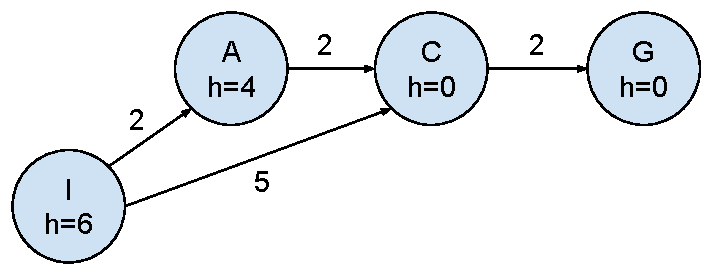
\includegraphics[width=0.8\textwidth]{fig/p3graph.pdf}
				\caption{$I$ and $G$ are the initial and goal states, respectively.}
				\label{fig:p3graph}
			\end{figure} \\
			\begin{table}[h]
				\centering
				%\begin{tabular}{c|c|c}
				\begin{tabular}{c|c}
					Expansion & Open List \\ %& Closed List \\
					\hline
%					1 & $[(I; 0+6)]$ & $[]$ \\
%					2 & $[(I,A; 2+4), (I,C; 5+0)]$ & $[(I,0)]$ \\
%					3 & $[(I,A; 2+4), (I,C,G; 5+2)]$ & $[(I,0),(C,5)]$ \\
%					4 & $[(I,A,C; 4+0), (I,C,G; 5+2)]$ & $[(I,0),(C,4),(A,2)]$ \\
%					5 & $[(I,A,C,G; 6+0), (I,C,G; 5+2)]$ & $[(I,0),(C,4),(A,2),(G,6)]$ \\
%					4 & $[(I,C,G; 5+2)]$ & $[I,C]$ \\
					1 & $[(I; 0+6)]$ \\
					2 & $[(I,C; 5+0), (I,A; 2+4)]$ \\
					3 & $[(I,A; 2+4), (I,C,G; 7+0)]$  \\
					4 & $[(I,A,C; 4+0), (I,C,G; 7+0)]$  \\
					5 & $[(I,A,C,G; 6+0), (I,C,G; 7+0)]$ \\
				\end{tabular}
				\caption{Execution trace of A$^*$ on the graph in Figure~\ref{fig:p3graph}. Nodes are given symbolically as $(path; g+h)$.}% of A$^*$ implemented with duplicate handling that does not remember cost information in the closed list.}
				\label{tbl:trace}
			\end{table}
		\item Is your heuristic function consistent? Is it generally possible to create such an example when the heuristic is consistent? Explain your answer.

			\vspace{0.25cm}
			My heuristic is inconsistent. $h(A) = 4 \nleq cost(A,C) + h(C) = 2$.
			
			In general it is impossible to create an example with a consistent heuristic.
			Let $i$, $n$, and $n'$ be nodes.
			Let $a_1$, $a_2$, $a_3$ be actions.
			Let $cost(i,a_1,n)+cost(n,a_3,n') < cost(i,a_2,n')$, but $cost(i,a_1,n)+h(n) > cost(i,a_2,n')+h(n')$,
			which creates the situation described.
			Since $cost(i,a_1,n)+cost(n,a_3,n') < cost(i,a_2,n')$ and all costs are non-negative,
			$cost(i,a_1,n) < cost(i,a_2,n')$.
			Then for $cost(i,a_1,n)+h(n) > cost(i,a_2,n')+h(n')$, $h(n) > h(n')$.
			This is not possible by the definition of consistency $h(n) \le cost(n,a_3,n')+h(n')$, when costs are non-negative.
		\item In general, will A$^*$ still find the optimal solution when this happens (i.e., a node is expanded with a g-value greater than the shortest distance from the initial state)?
			State clearly the assumptions you make about handling duplicate states.
			
			\vspace{0.25cm}
			A$^*$ will still find the optimal solution if no duplicate checking is implemented, or if a node representing
			a path from the start state $I$ to some other state $S$ with cost $C$ is not placed on the open list only if there
			exists some other node from $I$ to $S$ with cost $C'\le C$ that was already placed on the open list.
\end{enumerate}
\end{problem}
\begin{problem}{4}
	In this exercise, we consider the choice between two admissible heuristic functions, one of which is always at least as accurate as the other.
	More precisely, for a fixed goal, let $h_1$ and $h_2$ be two admissible heuristic functions such that $h_1(n) \le h_2(n)$ for every node n in the search tree.
	Now recall that the A$^*$ algorithm expands nodes according to their f values, but the order in which nodes of equal f values are expanded can vary, depending on the implementation.
	For a given heuristic function h, we say that an ordering of the nodes in the search tree is \textbf{h-legal} if expanding the nodes in that order is consistent with A$^*$ search using h.
	Let N denote the set of nodes expanded by an A* search using $h_1$ (the ``less accurate'' heuristic function).
	Prove that there is always some search ordering that is $h_2$-legal that expands only a (not necessarily strict) subset of the nodes in N.
	That is, prove that it is always possible that $h_2$ leads to a smaller search space than $h_1$.
	(Note that the question asks you to find some search ordering such that certain properties hold.
	Hint: It is not possible, in general, to show that these properties hold for an arbitrary search ordering.)

	\vspace{0.25cm}
	Let $r(n)$ be the remaining cost from node $n$ to the optimal solution.
	Let an implementation of A$^*$, $a$, break $f$ ties by imposing a descending ordering of the function $o(n)=r(n)-h(n)$.
	Therefore, in the event of $f$ ties, $a$ will expand the greatest underestimates of the true remaining cost first.
	Now consider nodes $n_1,\dots,n_m$ where $f(n_i)=f(n_j)$, $o(n_1) > \dots > o(n_m)$, and $n_m$ is on the solution path.
	$a$ using $h_1$ must expand $n_1,\dots,n_{m-1}$, but $a$ using $h_2$ may not expand them since $f_{h_1}(n_i) < f_{h_2}(n_i)$---meaning they are no longer tied with the node on the solution path.
	This is certainly true in the case where $n_m$ is a solution.
\end{problem}
\begin{problem}{5}
	A knight moves on a chessboard two squares up, down, left, or right followed by one square in one of the two directions perpendicular to the first part of the move (i.e., the move is L-shaped).
	Suppose the knight is on an unbounded board at square (0,0) and we wish to move it to square (x,y) in the smallest number of moves.
	(For example, to move from (0,0) to (1,1) requires two moves. The knight can move to board locations with negative coordinates.) 
	\begin{enumerate}
		\item Explain how to decide whether the required number of moves is even or odd without constructing a solution.

			\vspace{0.25cm}
			If $x \bmod 2 \neq y \bmod 2$, then the number of moves is odd. Otherwise, it is even.
		\item Design an admissible heuristic function for estimating the minimum number of moves required; it should be as accurate as you can make it.
			Prove rigorously that your heuristic is admissible.

			\vspace{0.25cm}
			The heuristic returns a lookup in a pattern database if it exists, otherwise a calculated underestimate.
			The pattern database contains the exact path cost to move from $(0,0)$ to $(x,y)$ where $x$ and $y$ are integers less than or equal to 3.
			These path costs were found by uniform cost search (UCS).
			Therefore, they do not over estimate the path cost, since UCS is optimal.
			Let $(x_g,y_g)$ and $(x, y)$ be the coordinates of the goal and the current position, respectively.
			A lookup key for the pattern database is $(|x_g-x|,|y_g-y|)$.
			The differences shift the problem to the origin.
			The absolute values translate the position to the first quadrant, which does not change path costs, since the problem is symmetric.

			The calculated heuristic is achieved by relaxing the problem and finding the admissible solution to that relaxed problem, making it an admissible heuristic to the original one.
			Instead of restricting the knight's movement to ``two squares up, down, left, or right followed by one square in one of the two directions perpendicular to the first part of the move'',
			it is allowed to move three times.
			Each time the knight may move up, down, left, or right one square.
			Therefore, the optimal path cost is at least $\lfloor\frac{m}{3}\rfloor$, where $m$ is the Manhattan distance.
		\item Implement A$^*$ and use it to solve the problem using your heuristic.
			Create two scatter plots showing (a) the number of nodes expanded as a function of solution length, and (b) computation time as a function of solution length for a set of randomly generated problem instances. 

			\vspace{0.25cm}
			Figure~\ref{fig:p5graph} shows both nodes exanded and computation time as a function of solution length.
			As expected, nodes expanded is highly correlated with computation time.
			\begin{figure}[h]
				\centering
				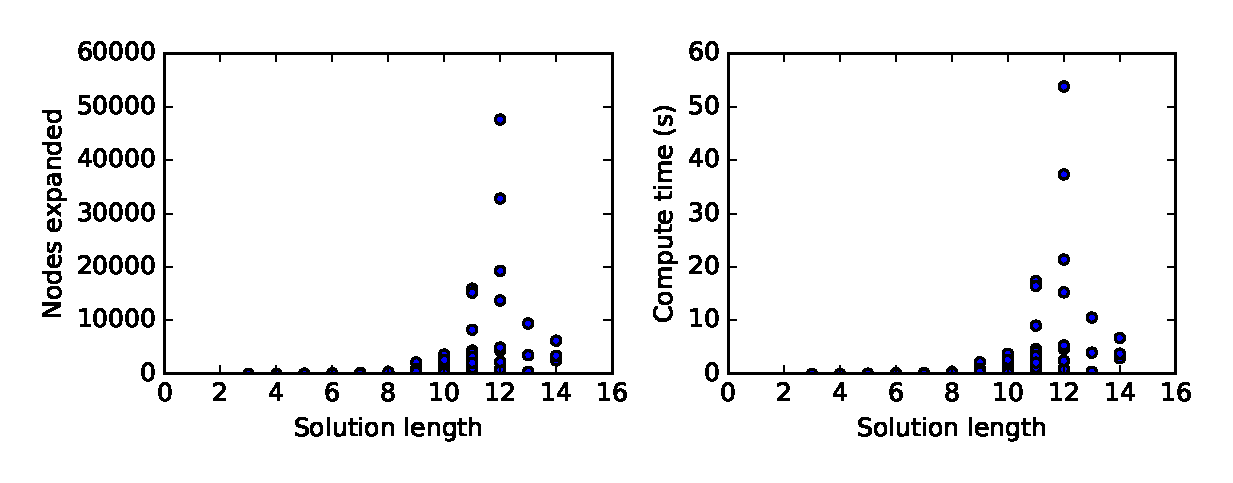
\includegraphics[width=0.8\textwidth]{fig/p5_h_4_max_20_iter_100_seed_0.eps}
				\caption{Nodes expanded and compute time as a function of solution length during 100 A$^*$ searches of randomly chosen goals in the 40-unit square.}
				\label{fig:p5graph}
			\end{figure}
	\end{enumerate}
\end{problem}
\begin{problem}{6}
	The Traveling Salesman Problem (TSP) is one of the most intensively studied computational problems.
	You can read about the history and applications of TSP algorithms at http://www.tsp.gatech.edu/.
	A TSP can be solved using heuristic search.
	One possible heuristic is the minimum spanning tree (MST), which can be used to estimate the cost of completing the tour, given that a partial tour has already been constructed.
	The MST cost of a set of cities is the smallest sum of the link costs of any tree that connects all the cities.
	\begin{enumerate}
		\item Formulate the TSP as a search problem and show that the MST heuristic can be derived from a relaxed version of the TSP.
			\begin{description}
				\item[States] Given a particular starting city, a state is any partial or complete tour beginning with that city.
				\item[Initial state] The salesperson begins the tour in a randomly selected initial city from the set of cities to be visited.
				\item[Actions] The actions consist of choosing which city to visit next from the set of unvisited cities, if that set's size is greater than two.
					Otherwise, choose the last unvisited city and complete the tour by continuing to the first visited city.
				\item[Succesors] The successors of a partial tour are all tours reachable by visiting one more unvisited city.
				\item[Path] The path is the sequence of visited cities.
				\item[Step cost] The distance between the last city in parent partial tour and the last city in its successor tour.
				\item[Path cost] The cost of a path is the sum of all distances between cities on the tour.
				\item[Goal test] The goal state consists of a path containing all cities with no repeated cities except the first and last city are the same.
			\end{description}
		\item Write a problem generator for instances of TSP where cities are represented by random points in the unit square (i.e., each coordinate is between 0 and 1).
			The number of cities to be generated should be a parameter.

			Please see the generateProblem function in p6.py.
		\item
			Find an efficient algorithm in the literature for constructing the MST, and use it with A* search to solve instances of the TSP (The two common algorithms are Prim's algorithm and Kruskal's algorithm); measure and plot the number of nodes expanded and computation time as a fuction of the number of cities for randomly generated problem instances.
			(Use problem instances that your algorithm can solve in less than a few minutes.)

			The portion of Prim's algorithm necessary to return the weight of the MST is implemented in function primMstWeight in p6.py.
			Nodes expanded and computation time as a function of the number of cities is given in Figure~\ref{fig:p6graph}.
			\begin{figure}[h]
				\centering
				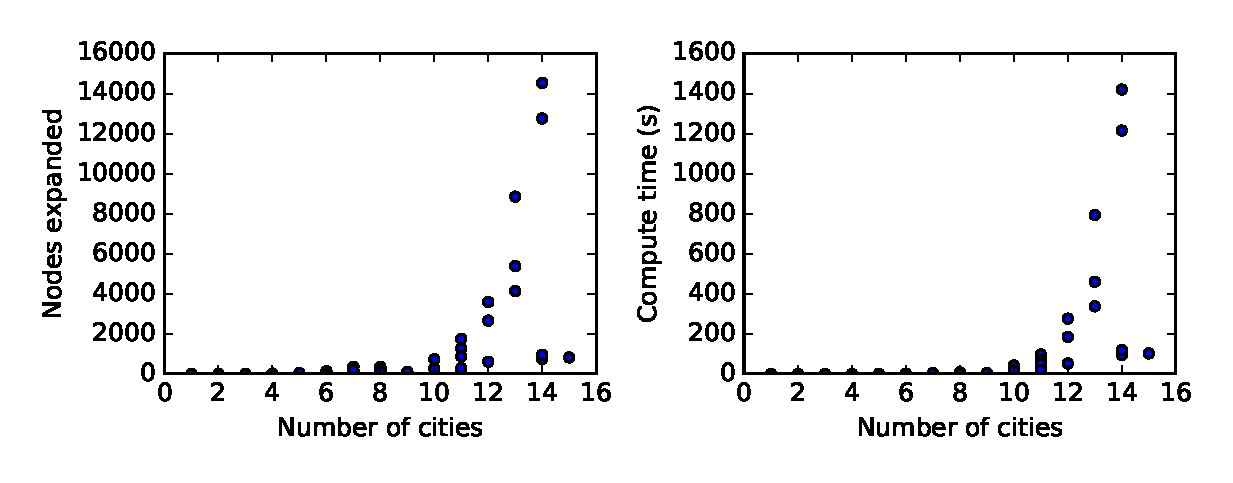
\includegraphics[width=0.8\textwidth]{fig/p6_h_0_cities_15_rand_True_iter_50_seed_0.eps}
				\caption{Nodes expanded and compute time as a function of the number of cities to be toured during 50 A$^*$ searches. The number of cities is a uniform random number between 1 and 15.}
				\label{fig:p6graph}
			\end{figure}
		\item[6.] blah
	\end{enumerate}
\end{problem}

\end{document}
